% !TeX root = ../main.tex

\chapter{相关技术理论}

本章节主要介绍系统实现以及使用过程中涉及到的相关技术,首先作为web端的系统平台,需要一些后台开发技术的支持,包括SpringBoot、
MyBatis、Mysql、Nginx等,其次数据湖分析系统作为大数据管理平台,一些数仓数据湖的架构体系和相关的开源技术组件是必不可少的,
其中包括传统离线数仓架构、实时数仓架构、数据湖架构和相关开源技术组件等。下面对相关技术进行简要介绍。

\section{后台开发相关技术}

基于Iceberg的数据湖分析系统使用的到的后台开发技术包括后端框架、持久化框架、关系型数据库和负载均衡等。

\subsection{SpringBoot}

基于Iceberg的数据湖分析平台采用SpringBoot作为后端开发框架。
SpringBoot 是 Pivotal 团队在 Spring 的基础上提供的一套全新的开源框架,
其目的是为了简化 Spring 应用的搭建和开发过程。SpringBoot 去除了大量的 XML 配置文件,简化了复杂的依赖管理。
SpringBoot 具有 Spring 一切优秀特性,Spring 能做的事,SpringBoot 都可以做,而且使用更加简单,
功能更加丰富,性能更加稳定而健壮。SpringBoot的出现带来全新的平台开发体验,降低了后端开发技术的使用门槛,具有以下优点:

(1)可快速构建独立的Spring应用

在构建SpringBoot项目时,只要根据需求选择对应的场景依赖,SpringBoot会自动添加该场景所需要的全部依赖并提供
自动化配置,在无需额外手动添加配置的情况下可以快速构建出一个独立的Spring应用程序。

(2)提供依赖启动器简化构建配置

在SpringBoot项目构建过程中,无需准备各种独立的JAR文件,只需在构建项目时根据开发场景需求选择对应的依赖启动器"starter"即可,
在引入的依赖启动器"starter"内部已经包含了对应开发场景所需的依赖,并会自动下载和拉取相关JAR包。例如,在Web开发时,只需在构建
项目时选择对应的Web场景依赖启动器spring-boot-starter-web,SpringBoot项目便会自动导入spring-webmvc、spring-web、
spring-boot-starter-tomcat等子依赖,并自动下载和拉取Web开发需要的相关JAR包。

(3)提供生产就绪功能

SpringBoot提供了一些用于生产环境运行时的特性,例如指标、健康检查和外部化配置。其中,指标和监控检查可以很方便的帮助
运维人员在运维期间监控项目运行情况;外部化配置可以很方便的让运维人员快速、方便的外部化配置和部署工作。

(4)极少的代码生成和XML配置

SpringBoot框架内部已经实现了与Spring以及其他常用第三方库的整合连接,并提供了默认最优化的整合配置,
使用时基本上不需要额外生成配置代码和XML配置文件。在需要自定义配置的情况下,SpringBoot更加提倡使用
Java config(Java配置类)替换传统的XML配置方式,这样更加方便查看和管理。

除此之外,SpringBoot 还实现了类与 Spring security、Spring data 等项目的无缝
集成,方便日后项目升级与扩展。基于以上综合考虑,选择SpringBoot作为后端框架。

\subsection{MyBatis}

MyBatis是一个Java持久化框架,它通过XML描述符或注解把对象与存储过程或SQL语句关联起来,映射成数据库内对应的纪录。
与其他对象关系映射框架不同,MyBatis没有将Java对象与数据库表关联起来,而是将Java方法与SQL语句关联。
MyBatis允许用户充分利用数据库的各种功能,例如存储过程、视图、各种复杂的查询以及某数据库的专有特性。
与JDBC相比,MyBatis简化了相关代码:SQL语句在一行代码中就能执行。MyBatis提供了一个映射引擎,
声明式的把SQL语句执行结果与对象树映射起来。
而且MyBatis与Spring Framework和Google Guice集成,这使开发者免于依赖性问题。

MyBatis支持声明式数据缓存(declarative data caching)。当一条SQL语句被标记为“可缓存”后,
首次执行它时从数据库获取的所有数据会被存储在一段高速缓存中,今后执行这条语句时就会从高速缓存中读取结果,
而不是再次命中数据库。

\subsection{Mysql}

MySQL是一个关系型数据库管理系统,由瑞典MySQL AB公司开发,目前属于Oracle旗下产品。
MySQL所使用的SQL语言是用于访问数据库的最常用标准化语言。MySQL软件采用了双授权政策,
分为社区版和商业版,由于其体积小、速度快、总体使用成本低,尤其是开放源码这一特点,
一般中小型网站都选择MySQL作为网站数据库。与其他的大型数据库例如 Oracle、DB2、SQL Server等相比,
MySQL自有它的不足之处,但是这丝毫也没有减少它受欢迎的程度。对于一般的个人使用者和中小型企业来说,
MySQL提供的功能已经绰绰有余,而且由于 MySQL是开放源码软件,因此可以大大降低总体拥有成本。

\section{传统离线数仓架构}

数据仓库概念是 Inmon 于1990年提出并给出了完整的建设方法。
数据仓库作为数据分析的重要体系架构,是一个面向主题的(Subject Oriented)、集成的(Integrate)、相对稳定的(Non-Volatile)
、反映历史变化(Time Variant)的数据集合,用于支持管理决策。
随着互联网时代来临,数据量暴增,大部分企业开始使用大数据工具 来替代经典数仓中的传统工具。
此时仅仅是工具的取代,架构上并没有根本的区别,可以把这个架构叫做传统离线数仓架构。
离线数仓,其实简单点来说,就是原来的传统数仓,数据以T+1的形式计算好放在那里,
给前台的各种分析应用提供算好的数据。到了大数据时代,这种模式被称为"大数据的批处理"。

数据源通过离线的方式导入到离线数仓中。下游应用根据业务需求直接读取想要的数据或加一层数据服务,比如MySQL或Redis。
数据仓库从模型层面可分为五层:

(1)ODS(Operation Data Store)

操作数据层,所有进入数据的数据首先会接入ODS层。一般来说ODS层的数据是多复杂多样的。从数据粒度上看ODS层是粒度最细的数据层。

(2)DWD(Data Warehouse Details)

数据仓库明细层,数据明细层的数据应是经过ODS清洗,转后的一致的、准确的、干净的数据。DWD层数据粒度通常和ODS的粒度相同,不同的是该层的数据质量更高,字段更全面等。在数据明细层会保存BI系统中所有的历史数据,例如保存近10年来的数据。

(3)DWM(Data Warehouse middle)

数据中间层,在DWD的基础上进行轻微的聚合操作,算出相应的统计指标。

(4)DWS(Data warehouse service)

数据服务层,该层数据是面向主题来组织数据的,通常是星形或雪花结构的数据。从数据粒度来说,这层的数据是轻度汇总级的数据,已经不存在明细数据了。

(5)ADS(Application data service)

数据应用层,它是完全为了满足具体的分析需求而构建的数据,也是星形或雪花结构的数据。从数据粒度来说是高度汇总的数据。其汇总的目标主要是按照应用需求进行的。

\section{实时数仓架构}

随着大数据应用的发展,人们逐渐对系统的实时性提出了要求,对于传统离线数仓,
数据从接入直到展示存在着小时级以上的延迟,这其中一方面是因为批处理框架本身延迟的限制,另一方面也是因为对于变化数据捕捉能力的缺失:

(1)无法避免的架构延迟

当前数仓的ETL入库过程通常是基于批的方式,数据按小时、天等的粒度导入到数据仓库中,
由于ETL的复杂度和固有的延迟,导致端到端的时延被放大到T+1;
数仓构建中的层次化划分和处理——原始层、明细层、汇总层、应用层——也在一定程度上增加了最后数据展示的延迟。

(2)高昂的数据修改成本

对于延迟数据的修正,以及近似数据的修正在传统的基于Hive的数仓中是一个非常高代价的操作,
Hive需要将相应的分区或文件读出来更新后重新写回到表中(即使只有一行数据的修改),而这在无形中也加剧了整体的时延。

为了解决现有数仓架构的时延问题,业界也在该领域进行了较多的探索,其中最主要的探索是Lambda架构和Kappa架构。

\subsection{Lambda 架构}

Lambda架构是一种常见的数据处理体系结构,它的数据的处理依赖流式计算层(Streaming Layer)
和批处理计算层(Batch Layer)的双重计算。每隔几个小时,批处理过程被启动以计算精确的业务状态,
并将批量更新加载到服务层(Serving Layer)。同时,为了消除上述几个小时的等待时间,会在流式
计算层对这个业务数据进行实时的状态更新。然而,这个流计算的状态只是一个最终结果的近似值,
最终需要被批处理的计算结果所覆盖。Lambda架构图如图2.1所示。

\begin{figure}[h]
  \centering
  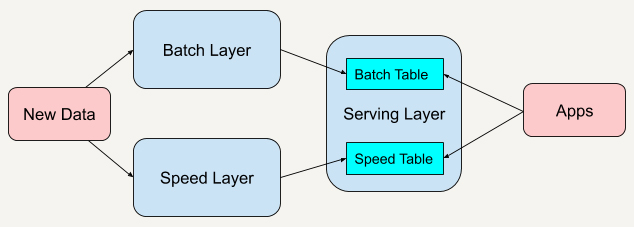
\includegraphics[width=1.0\textwidth]{Lambda.png}
  \caption{Lambda架构图}
  \label{fig:badge}
\end{figure}

可以看到,为了达到Velocity(近实时的计算),用户需要设计一个非常复杂的架构。
首先,需要维护流式计算层和批处理计算层两种框架,两种框架的差异性造成了极大的维护成本。
其次,两种计算框架的实现的差异造成了需要维护不同的代码来服务两层应用,增加开发和维护成本。
同时由于两种模式提供的状态差异,需要为批处理和流处理提供不同的服务层,并在这个上面再做合并抽象,或者设计应用一个相当复杂的服务系统。
数据存在多个不同的源中,容易造成数据的不一致出现。

为了解决Lambda架构的复杂性,也出现有了诸多的改进方案,比如Kappa架构及其变种。

\subsection{Kappa 架构}

现有的流式框架和消息中间件可以非常快地增加并行度,以及重播历史来处理重新处理实时数据,
避免在实时数据处理系统上再"粘上"一个离线数据处理系统。由此提出了Kappa架构。

Kafka或者其他消息中间件,具备保留多日数据的能力。正常情况下Kafka都是吐出实时数据,
经过实时处理系统,进入服务数据库(Serving DB)。当系统需要数据订正时,重放消息,
修正实时处理代码,扩展实时处理系统的并发度,快速回溯过去历史数据。Kappa架构图如图2.2所示。

\begin{figure}[h]
  \centering
  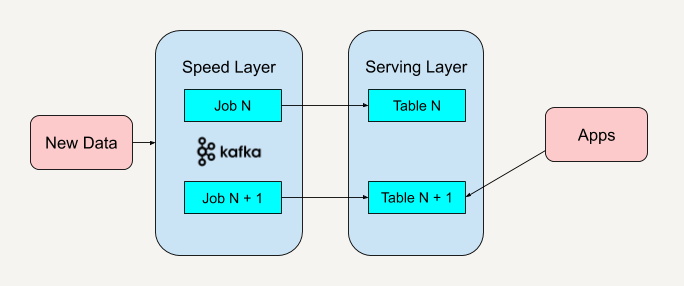
\includegraphics[width=1.0\textwidth]{Kappa.png}
  \caption{Kappa架构图}
  \label{fig:badge}
\end{figure}

可以看到,这样的架构简单,避免了维护两套系统还需要保持结果一致的问题,也很好解决了数据订正问题。但它也有它的问题,
其一是消息中间件缓存的数据量和回溯数据有性能瓶颈,举个例子,假定算法需要过去180天的数据,如果都存在消息中间件,
无疑有非常大的压力,同时,一次性回溯订正180天级别的数据,对实时计算的资源消耗也非常大;
其二是在实时数据处理时,遇到大量不同的实时流进行关联时,非常依赖实时计算系统的能力,很可能因为数据流先后顺序问题,导致数据丢失。

\section{数据湖架构}

数据湖是一种以原生格式存储各种大型原始数据集的数据存储库。您可以通过数据湖宏观了解自己的数据。
在一些需要为数据设置大型整体存储库的企业中,数据湖正在成为一种更通用的数据管理策略。
原始数据是指尙未针对特定目的处理过的数据。数据湖中的数据只有在查询后才会进行定义。
数据科学家可在需要时用比较先进的分析工具或预测建模法访问原始数据。
数据湖可为您保留所有数据,在您存储前,任何数据都不会被删除或过滤。有些数据可能很快就会用于分析,
有些则可能永远都派不上用场。有些数据也可能为了不同用途而多次使用,同时也有数据会为了特定目的不断优化,
这就让我们难以用不同的方式重复使用数据。

Pentaho 的首席技术官 James Dixon 对"数据湖"进行了介绍。之所以将其称为湖,是因为这种数据存储库
可以在自然状态下存储大量数据,就像一片未经过滤或包装的水体。数据从多种来源流入湖中,然后以原始格式存储。
只有在需要用来分析时,数据湖中的数据才会进行转换,
因而分析数据时需要用到数据库模式(Schema)。这叫作"读时模式",因为数据会一直处于原始状态,直到读取使用。

通过数据湖,用户能够以自己的方式访问和探索数据,无需将数据移入其他系统。不同于定期从其他平台或数据
存储库提取分析报告,数据湖的分析和报告通常可以临时获取。但是,用户可在必要时通过Schema和自动化复制报告。
对于数据湖中的数据,您需要监管和持续维护,才能确保数据时刻可用和可访问。如果维护不当,您的数据就可能会沦为一堆垃圾,
无法访问、难以操作、价格高昂而且毫无用处。用户无法访问的数据湖,就成了"数据沼泽"。

数据湖采用扁平化架构,因为这些数据既可能是非结构化,也可能是半结构化或结构化,
而且是从组织内的各种来源所收集,而数据仓库则是把数据存储在文件或文件夹中。数据湖可托管于本地或云端。
鉴于其架构特点,数据湖可大规模扩展,能达到艾字节。这一点很重要,因为创建数据湖时,
您通常并不知道需要保存的数据量。传统数据存储系统就无法以这种方式扩展。
这种架构可以大大方便了数据科学家,因为他们可以通过这种架构挖掘和探索企业的数据,
并共享和相互参照数据(包括不同领域的异构数据),以便进行提问并找到新的分析。他们还可以利用大数据分析和机器学习分析数据湖中的数据。
虽然数据在存入数据湖之前没有固定的模式,但利用数据监管,你仍然可以有效避免出现数据沼泽。

数据湖示意图如图2.3所示:

\begin{figure}[h]
  \centering
  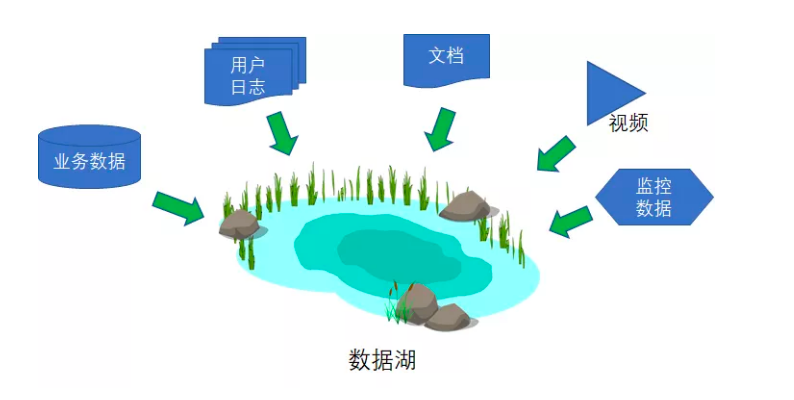
\includegraphics[width=1.0\textwidth]{dataLake.png}
  \caption{数据湖示意图}
  \label{fig:badge}
\end{figure}

\section{相关开源技术组件}

本小节主要介绍和本系统构建相关的几个核心开源组件,除了下述讨论的几个组件外,本系统在实现或者使用中
还涉及到了Hadoop、Presto、Parquet、Hive、Zookeeper、Kafka、Flink CDC等大数据体系中常见的开源技术组件,因篇幅所限,
这里不再一一展开讨论。

\subsection{Apache Iceberg}

随着数据湖在大数据领域的流行,越来越多的公司开始使用 Iceberg 搭建统一的湖仓平台。
Iceberg是一种表格式(table format),我们可以简单理解为它是基于计算层(flink、spark)
和存储层(orc、parquet)的一个中间层,我们可以把它定义成一种"数据组织格式",Iceberg将其称之为"表格式"也是表达类似的含义。

数据格式顾名思义就是数据的存储格式。在大数据领域,随着对于性能的追求,
数据格式也在不停地进化,从TXT File,CSV File,Json File,Sequence File
等行式存储格式,到后期的RCFile,Parquet,ORC等列式存储格式。它们所表示的是在一个文件中数据是如何存储的。
在整个大数据软件栈中,Data Format所处的位置如图2.4如所示:

\begin{figure}[h]
  \centering
  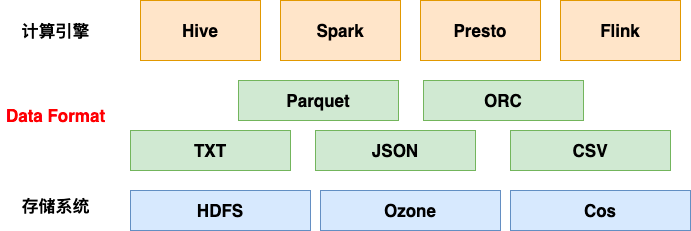
\includegraphics[width=1.0\textwidth]{DataFormat.png}
  \caption{Data Format示意图}
  \label{fig:badge}
\end{figure}

数据格式所表示的是一个文件中数据的存储格式,而对于一张Hive表来说,它通常包含了多个文件,为了更好地利用HDFS这样的分布式文件系统进行文件过滤,
Hive表利用目录的方式来组织表:一张表映射到HDFS上是一个目录,目录中可以包含子目录,而子目录的定义是分区信息,
数据按分区列写入到不同的目录中,查询引擎据分区条件找到相应的目录。因此说,"以目录的方式来组织数据成为一张表"
是一种较为朴素的表组织方式,称为表格式。
而Iceberg的出现,试图打破现在这种朴素的表组织方式,定义了一种非目录形式的表组织方式,Table Format所处的位置如图2.5如所示:

\begin{figure}[h]
  \centering
  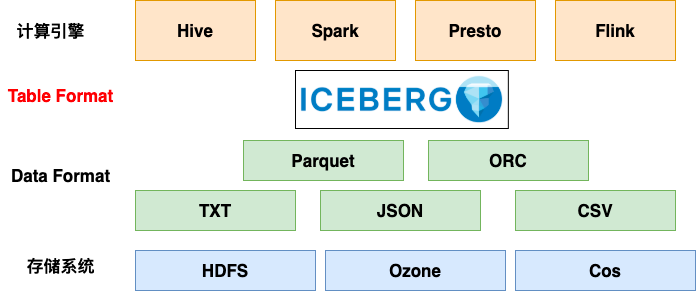
\includegraphics[width=1.0\textwidth]{TableFormat.png}
  \caption{Table Format示意图}
  \label{fig:badge}
\end{figure}

因此,Iceberg是一种表格式,Iceberg定义了表中文件的组织方式,而不是一个文件中数据的格式;
是一个库,Iceberg是一个库,通过和计算引擎一起运行将表以Iceberg的组织方式写入到底层存储系统中。而不是一个独立的服务(不涉及部署);
是一个开放标准,Iceberg定义了一个开放的表格式,并在其上设计了一套引擎无关的API,因此任何引擎只要适配了Iceberg的API都可以读写Iceberg表。

\subsection{Apache Flink}

Flink是一个批处理和流处理结合的统一计算框架,其核心是一个提供了数据分发以及并行化计算
的流数据处理引擎。它的最大亮点是流处理,是业界最顶级的开源流处理引擎。
Flink最适合的应用场景是低时延的数据处理场景:高并发pipeline处理数据,时延毫秒级,且兼具可靠性。

Flink的架构如图2.6所示:

\begin{figure}[h]
  \centering
  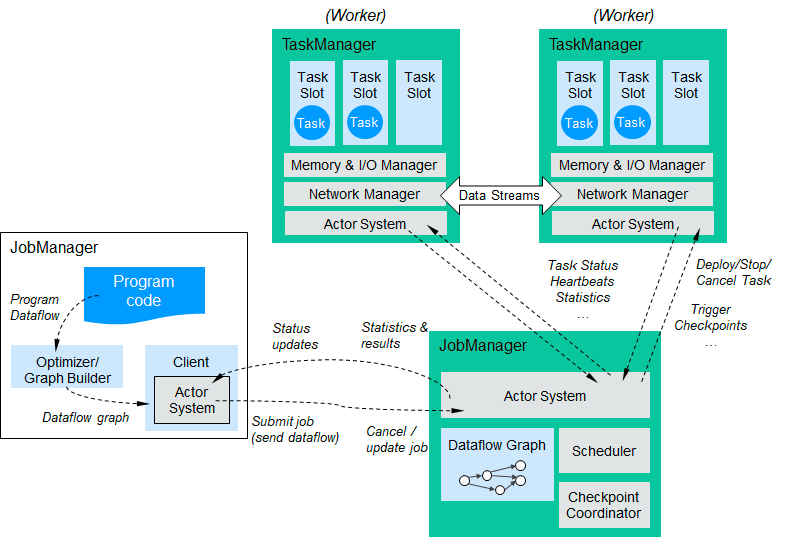
\includegraphics[width=1.0\textwidth]{Flink.png}
  \caption{Flink架构图}
  \label{fig:badge}
\end{figure}

Flink整个系统包含三个部分:

(1)Client

Flink Client主要给用户提供向Flink系统提交用户任务(流式作业)的能力;

(2)TaskManager

Flink系统的业务执行节点,执行具体的用户任务。TaskManager可以有多个,各个TaskManager都平等;

(3)JobManager

Flink系统的管理节点,管理所有的TaskManager,并决策用户任务在哪些TaskManager执行。JobManager在HA模式下可以有多个,但只有一个主JobManager。

\subsection{Apache Spark}

Spark是一个用于分布式数据处理和并行计算的开源项目,最早由UC Berkeley 的AMP实验室开发,
现在已经交由Apache开源项目组管理。Spark目前变得非常流行,跟其高效性,通用性和易于编程性
都有很大关系。Spark在机器学习,大数据处理和实时数据处理,以及分布式的应用场景中都能充分发挥作用。
Apache Spark 所具有的众多优点使其成为 Hadoop 生态系统中最活跃的项目之一,其中包括:

(1)快速

通过内存中缓存和优化的查询执行方式,Spark 可针对任何规模的数据进行快速分析查询;

(2)开发人员友好

Apache Spark 原生支持 Java、Scala、R 和 Python,可为您提供多种应用程序构建语言。
这些 API 让您的开发人员变得更轻松,因为它们可以将复杂的分布式处理隐藏在简单的高级操作符背后,从而大量减少所需的代码数量。

(3)多个工作负载

Apache Spark 自带运行多个工作负载功能,包括交互式查询、实时分析、机器学习和图形处理等。
一个应用程序可无缝与多个工作负载整合。

Spark架构如图2.7所示:

\begin{figure}[h]
  \centering
  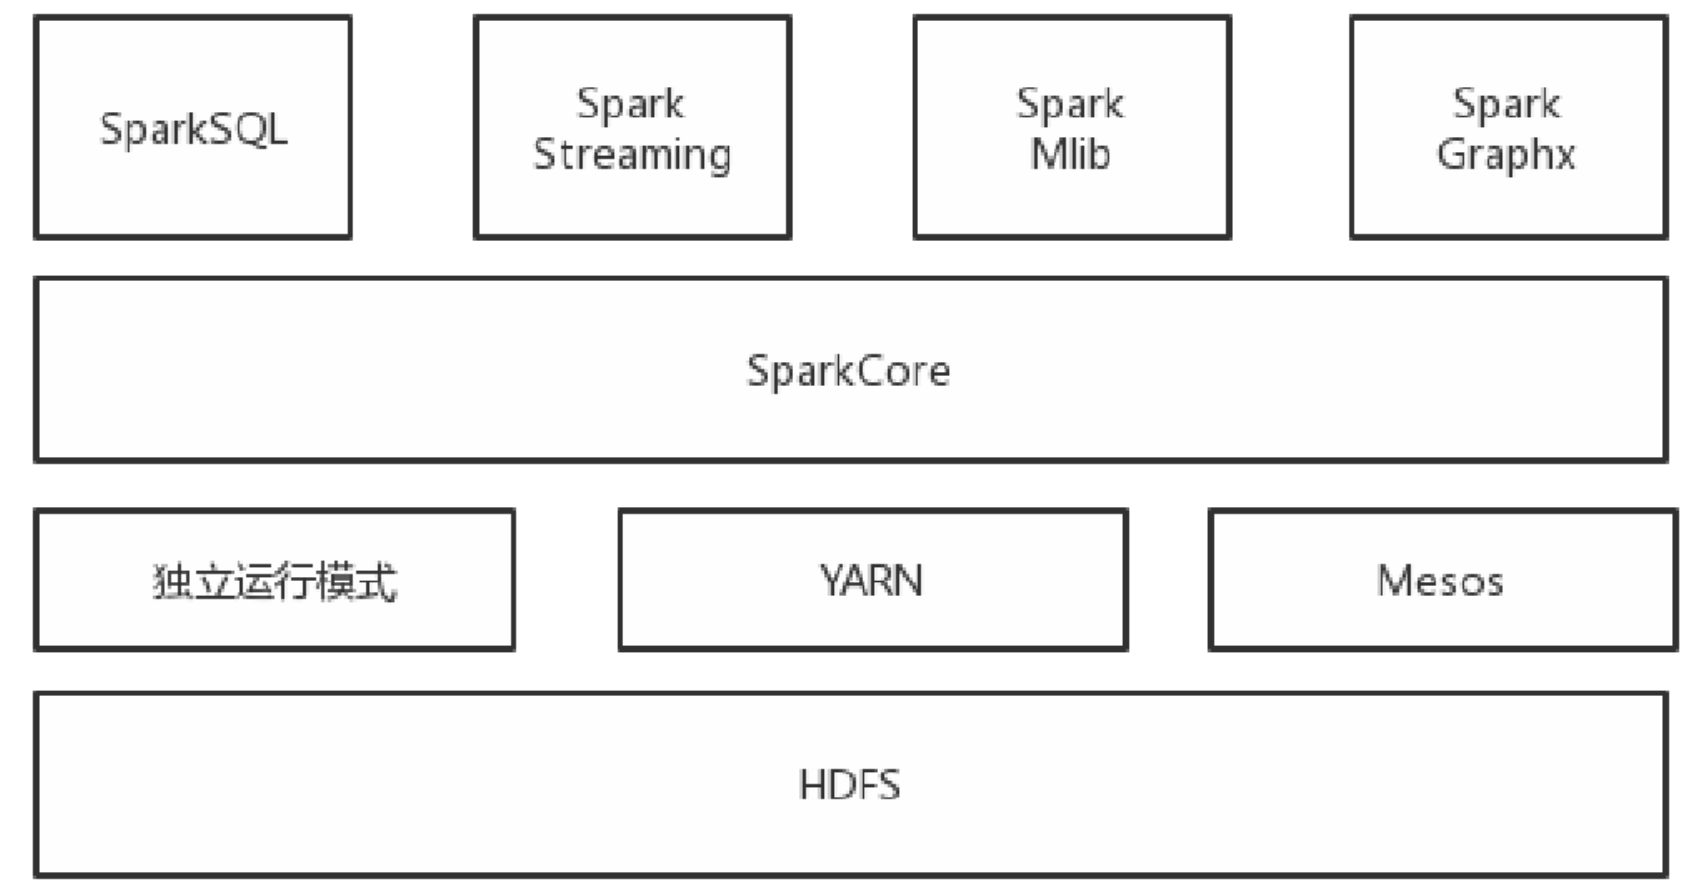
\includegraphics[width=1.0\textwidth]{spark.png}
  \caption{Spark架构图}
  \label{fig:badge}
\end{figure}

\subsection{Hive Metastore}

Hive Metastore 用于管理元数据(Metadata)并提供服务。 元数据是描述其它数据的数据[15],或者说是用于
提供某种资源的有关信息的结构数据(structured data)。这里的元数据包括:数据库、表、表的模式、目录、分区、索引以及命名空间等。

Hive Metastore默认是不做任何用户认证的,也就是说只要指定metastore服务的IP和端口就可以通过
Thrift协议连接上并读取元数据。Metastore也支持基于Kerberos的认证,不过这里的认证只是为了保护
对于metastore的访问,一旦认证通过,任何人调用相同api所获得的结果都是一样的,而不会管当前到底是谁在调用。

Hive Metastore架构如图2.8所示:

\begin{figure}[h]
  \centering
  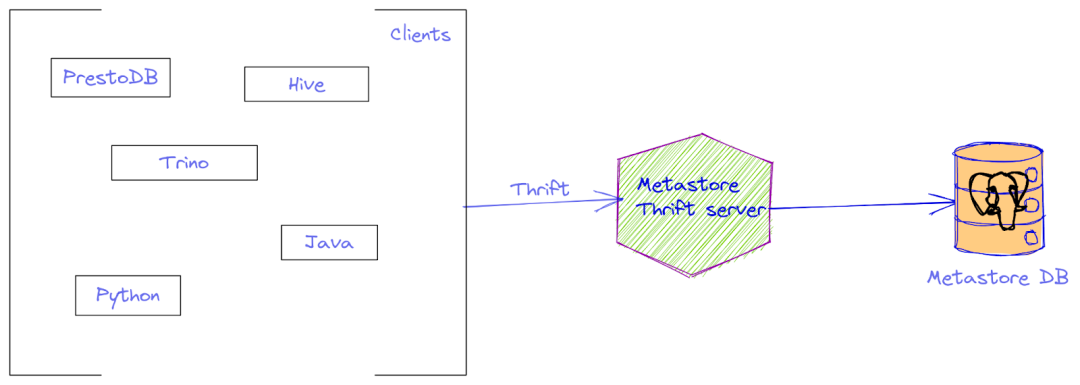
\includegraphics[width=1.0\textwidth]{HiveMetastore.png}
  \caption{Hive Metastore架构图}
  \label{fig:badge}
\end{figure}

\section{本章小结}

本章主要对数据湖分析系统在实现过程以及使用过程中用到的关键技术进行介绍。首先介绍了后台系统开发使用到的技术,包括SpringBoot、
mysql等,然后介绍了传统离线数仓模型、实时数仓模型、数据湖模型,最后介绍了相关的开源技术组件,这为后续的讨论打下了理论基础。
因篇幅有限,故而只讨论了几个比较核心的组件,后文将这些技术有机整合在一起,形成新一代的全场景实时数仓——数据湖分析系统。

